\documentclass[pdf]{beamer}

%\usepackage{beamerthemesplit,multimedia}

\usetheme{Warsaw}

\usepackage{alltt}

%\usepackage{amssymb, amsmath,stmaryrd}
\usepackage{amssymb, amsmath}

\usepackage[english]{babel}

\usepackage{tikz}
\usetikzlibrary{calc,trees,positioning,arrows,chains,automata,shapes.geometric,%
    decorations.pathreplacing,decorations.pathmorphing,shapes,%
    matrix,shapes.symbols}

\usetikzlibrary{shapes,arrows,automata,positioning,calc}
\usetikzlibrary{fit,backgrounds}
\usetikzlibrary{decorations.pathreplacing}
\tikzset{
>=stealth',
  punktchain/.style={
    rectangle,
    rounded corners,
    % fill=black!10,
    draw=black, very thick,
    text width=6em,
    minimum height=3em,
    text centered,
    on chain},
  line/.style={draw, thick, <-},
  element/.style={
    tape,
    top color=white,
    bottom color=blue!50!black!60!,
    minimum width=8em,
    draw=blue!40!black!90, very thick,
    text width=10em,
    minimum height=3.5em,
    text centered,
    on chain},
  every join/.style={->, thick,shorten >=1pt},
  decoration={brace},
  tuborg/.style={decorate},
  tubnode/.style={midway, right=2pt},
}


%\usepackage{macros3}
\newcommand{\natplus}{\nat^{>0}}
\newcommand{\realsplus}{R^{\geq 0}}
\newcommand{\delays}{R^{> 0}}
\newcommand{\stoptimer}{\mathit{kill}}
\newcommand{\tosymbol}{\mathit{to}}
\newcommand{\toevent}[1]{\mathit{to}[#1]}
\newcommand{\toevents}{\mbox{\sl TO}}
\newcommand{\extinputs}{\hat{I}}
\newcommand{\acttimers}{\mathit{active}}
\newcommand{\Head}[1]{\mathsf{Head}({#1})}
\newcommand{\Tail}[1]{\mathsf{Tail}({#1})}
\newcommand{\Last}[1]{\mathsf{Last}({#1})}
\newcommand{\expirable}{\mathit{expirable}}
\newcommand{\tvals}{\kappa}
\newcommand{\Vals}[1]{\mathit{Val}({#1})}
\newcommand{\delay}[2]{t_{[#1:#2]}}
\newcommand{\timerof}[2]{x_{#1}^{#2}}
\newcommand{\constrof}[1]{\phi_{#1}}
\newcommand{\Post}{\mathsf{Post}}
\newcommand{\beh}{\mathit{beh}}
\newcommand{\untime}{\mathit{untime}}
\newcommand{\run}{\mathit{pullback}}
\newcommand{\timedword}{\mathit{tw}}

\newcommand{\conc}{\cdot}
\newcommand{\tuple}[1]{\langle #1\rangle}
\newcommand{\set}[1]{\lbrace #1\rbrace}
\newcommand{\vect}[2]{{#1}_1 , \ldots , {#1}_{#2}}
\newcommand{\setcomp}[2]{\set{#1 ~:~ #2}}
\newcommand{\domof}[1]{\dom(#1)}
\newcommand{\ranof}[1]{\ran(#1)}
\newcommand{\vars}{\mathcal{X}}
\newcommand{\varsof}[1]{\vars(#1)}
\newcommand{\ctimers}{X}
\newcommand{\remap}{\pi}
\newcommand{\remapinst}{\rho}
\newcommand{\normalize}{\gamma}
\newcommand{\normalizeof}[2]{\normalize_{#2}^{#1}}
\newcommand{\timerbij}{\gamma}
\newcommand{\timerequiv}{\pi}
\newcommand{\extendedby}{\lhd}
\newcommand{\uttrace}{\textsf{tr}}
\newcommand{\uttraceof}[1]{\uttrace(#1)}
\newcommand{\uttracesof}[1]{\textsf{Tr}(#1)}
\newcommand{\strace}{\textsf{tr}_s}
\newcommand{\ssuffix}{v_s}
\newcommand{\suftraces}{\textsf{Tr}_s}
\newcommand{\pinpof}[1]{\textit{inp}_p(#1)}
\newcommand{\sinpof}[1]{\textit{inp}_s(#1)}
\newcommand{\symbinpof}[1]{\textit{symbinp}(#1)}
\newcommand{\word}{w}
\newcommand{\smap}{{\cal O}}
\newcommand{\smappre}{{\cal O_p}}
\newcommand{\smapsuf}{{\cal O_s}}
\newcommand{\obspre}{{\cal O_U}}

% collection of macros used in the paper

%Learners
\newcommand{\learnlib}{LearnLib}

\newcommand{\A}{{\mathcal A}}
\newcommand{\B}{{\mathcal B}}
\newcommand{\CH}{{\mathcal H}}
\newcommand{\M}{{\mathcal M}}
\newcommand{\N}{{\mathcal N}}
\newcommand{\hypoof}[2]{\mathcal{H}(#1,#2)}

\newcommand{\nat}{{\mathbb N}}
\newcommand{\integers}{{\mathbb Z}}

\newcommand{\sem}[1]{[\kern-.5mm[{#1}]\kern-.5mm]}
\newcommand{\eqclass}[1]{[{#1}]}

%DOMAIN AND RANGE
\newcommand{\dom}{{\textsf{dom}}}
\newcommand{\ran}{{\textsf{ran}}}

\newcommand{\natplus}{\nat^{>0}}
\newcommand{\realsplus}{{\mathbb R}^{\geq 0}}
\newcommand{\delays}{{\mathbb R}^{> 0}}
\newcommand{\stoptimer}{\mathit{kill}}
\newcommand{\tosymbol}{\mathit{to}}
\newcommand{\toevent}[1]{\mathit{to}[#1]}
\newcommand{\toevents}{\mbox{\sl TO}}
\newcommand{\extinputs}{\hat{I}}
\newcommand{\Head}[1]{\mathsf{Head}({#1})}
\newcommand{\Tail}[1]{\mathsf{Tail}({#1})}
\newcommand{\Last}[1]{\mathsf{Last}({#1})}
\newcommand{\expirable}{\mathit{expirable}}
\newcommand{\tvals}{\kappa}
\newcommand{\Vals}[1]{\mathit{Val}({#1})}
\newcommand{\delay}[2]{d_{[#1:#2]}}
\newcommand{\timerof}[2]{x_{#1}^{#2}}
\newcommand{\Post}{\mathsf{Post}}
\newcommand{\beh}{\mathit{beh}}
\newcommand{\untime}{\mathit{untime}}
\newcommand{\run}{\mathit{pullback}}
\newcommand{\timedword}{\mathit{tw}}
\newcommand{\timedinputword}{\mathit{tiw}}
\newcommand{\untimedinputword}{\mathit{uiw}}
\newcommand{\startedby}{\mathit{startedby}}
\newcommand{\Mealy}{\mathit{Mealy}}
\newcommand{\finitesubsets}[1]{{\mathcal{P}}_{\mathit{fin}}(#1)}
\newcommand{\conc}{\cdot}
\newcommand{\tuple}[1]{\langle #1\rangle}
\newcommand{\set}[1]{\lbrace #1\rbrace}
\newcommand{\vect}[2]{{#1}_1 , \ldots , {#1}_{#2}}
\newcommand{\setcomp}[2]{\set{#1 ~:~ #2}}
\newcommand{\domof}[1]{\dom(#1)}
\newcommand{\ranof}[1]{\ran(#1)}
\newcommand{\can}[1]{\mathit{can}({#1})}
\newcommand{\uncan}[1]{\mathit{uncan}({#1})}
\newcommand{\zone}[1]{\mathit{Zone}({#1})}
\newcommand{\vars}{\mathcal{X}}
\newcommand{\varsof}[1]{\vars(#1)}
\newcommand{\remap}{\pi}
\newcommand{\remapinst}{\rho}
\newcommand{\constr}{\phi}


\newcommand{\emptyword}{\epsilon}
\newcommand{\lengthof}[1]{|#1|}
\newcommand{\true}{{\it true}}
\newcommand{\false}{{\it false}}

%% macros for ``approximation''
\newcommand{\acttimers}{\mathit{active}}
\newcommand{\constrof}[1]{\phi_{#1}}
\newcommand{\post}{\mathit{post}}

\newcommand{\ctimers}{X}
\newcommand{\normalize}{\gamma}
\newcommand{\normalizeof}[2]{\normalize_{#2}^{#1}}
\newcommand{\timerbij}{\gamma}
\newcommand{\timerequiv}{\pi}
\newcommand{\extendedby}{\lhd}
\newcommand{\uttrace}{\textsf{tr}}
\newcommand{\uttraceof}[1]{\uttrace(#1)}
\newcommand{\uttracesof}[1]{\textsf{Tr}(#1)}
\newcommand{\strace}{\textsf{tr}_s}
\newcommand{\ssuffix}{v_s}
\newcommand{\instancesof}[1]{[\![ #1 ] \! ]}
\newcommand{\suffixbehs}[3]{({#2}^{-1}{#1})\lceil{#3}}
\newcommand{\getmemorable}[3]{\mathit{mem}_{#1,#3}(#2)}
\newcommand{\getassignment}[3]{\mathit{val}_{#1,#3,#2}}
\newcommand{\feasibleinputs}[2]{\mathit{feas}_{#2}(#1)}
\newcommand{\extend}[3]{(#1 \xrightarrow{#2/#3} \emptyset)}
\newcommand{\suffbij}[2]{g_{|#1| \to |#2|}}
\newcommand{\suftraces}{\textsf{Tr}_s}
\newcommand{\pinpof}[1]{\textit{inp}_p(#1)}
\newcommand{\sinpof}[1]{\textit{inp}_s(#1)}
\newcommand{\symbinpof}[1]{\textit{symbinp}(#1)}
\newcommand{\word}{w}
%% \newcommand{\smap}{{\cal O}}
%% \newcommand{\smappre}{{\cal O_p}}
%% \newcommand{\smapsuf}{{\cal O_s}}
%% \newcommand{\obspre}{{\cal O_U}}


% Define various macros
\definecolor{darkgreen}{rgb}{0,.75,0}
\definecolor{darkred}{rgb}{.75,0,0}
\definecolor{darkblue}{rgb}{0,0,.75}
\newcommand{\red}[1]{\color{darkred}{#1}\normalcolor }
\newcommand{\green}[1]{\color{darkgreen}{#1}\normalcolor }
\newcommand{\blue}[1]{\color{blue}{#1}\normalcolor }
\newcommand{\tts}{\tt \footnotesize}
\newcommand{\ra}{\rightarrow}

\title[Learning Mealy Machines with Timers]{%
Learning Mealy Machines with Timers - Preliminary Report}

\author[Jonsson and Vaandrager]{%
Bengt Jonsson \and Frits Vaandrager}

\institute{Uppsala and Nijmegen}

\date[Grenoble]{Verimag, Grenoble, October 2017}

\beamertemplatenavigationsymbolsempty
%\beamertemplateshadingbackground{red!10}{blue!10}

\begin{document}

\frame{\titlepage}

%\section{Introduction}
\frame{
\frametitle{Motivation}

\blue{Timing behavior}\  plays a crucial role in applications of model learning to network protocols and legacy software, but existing tools cannot handle it. These tools only work for untimed, deterministic systems. There has been some work on algorithms for timed systems, e.g.,
\begin{itemize}
\item
Grinchtein, Jonsson \& Leucker. \green{Learning of event-recording automata}, TCS, 2010.
\item
Caldwel, Cardell-Oliver \& French. \green{Learning time delay Mealy machines}. IEEE TASE, 2016.
\item
Mens \& Maler. \green{Learning Regular Languages over Large Ordered Alphabets}. LMCS, 2015.
\end{itemize}
but these algorithms are not practical because of high complexity and/or limited expressivity.
}

\frame{
\frametitle{Timing Behavior in Network Protocols}
Sender alternating-bit protocol, adapted from Kurose \& Ross:

\vspace{1em}
\begin{tikzpicture}[->,>=stealth',shorten >=1pt,auto,node distance=3cm,main node/.style={circle,draw,font=\sffamily\large\bfseries}]
  \node[initial, state] (1) {$q_0$};
  \node[state] (2) [right of=1] {$q_1$};
  \node[state] (3) [below of=2] {$q_2$};
  \node[state] (4) [below of=1] {$q_3$};

  \path[every node/.style={font=\sffamily\scriptsize}]
    (1) edge [text width=1.5cm] node {$\mathit{in}/\mathit{send0}$ \\ $\mathit{start\_timer(3)}$} (2)
    (2) edge [text width=1.5cm] node {$\mathit{ack0}/\mathit{void}$ \\ $\mathit{stop\_timer}$} (3)
        edge [loop right, text width=1.5cm] node {$\mathit{to}/\mathit{send0}$\\ $\mathit{start\_timer}(3)$ } (2)
    (3) edge [text width=1.5cm] node {$\mathit{in}/\mathit{send1}$ \\ $\mathit{start\_timer(3)}$} (4)
    (4) edge [text width=1.5cm] node {$\mathit{ack1}/\mathit{void}$ \\ $\mathit{stop\_timer}$} (1)
        edge [loop left, text width=2cm] node {$\mathit{to}/\mathit{send1}$\\ $\mathit{start\_timer(3)}$} (4);
\end{tikzpicture}
}

\frame{
\frametitle{Idea}

Develop learning algorithm for model of Mealy machines with timers in which transitions may start, stop and restart multiple timers, and besides input events we also have timeouts.

}

\frame{
\frametitle{Formalizing Mealy machines with timers}
We assume an unbounded set $X$ of \red{timers}\  $x$, $x_1$, $x_2$, etc.\ 
For a set $I$, let $\extinputs$ be $I \cup \{ \toevent{x} \mid x \in X \}$.
A \red{Mealy machine with timers (MMT)}\  is a tuple
$\M = (I, O, Q, q_0, \vars, \delta, \lambda, \remap)$, where
\begin{itemize}
\item
$I$ is a finite set of input events,
\item
$O$ is a finite set of output events, 
%containing a special default output $\Lambda$,
\item
$Q$ is a finite set of states,
\item
$q_0 \in Q$ is the initial state,
\item
for each $q \in Q$ a finite set of timers $\varsof{q}$, with $\varsof{q_0} = \emptyset$,
\item
$\delta: Q \times \extinputs \hookrightarrow  Q$ is a transition function,
%with $\delta(q,i)$ defined iff $q \in Q$ and $i \in I \cup \{ \toevent{x} \mid x \in \varsof{q} \}$, 
\item
$\lambda: Q \times \extinputs \hookrightarrow O$ is an output function, 
\item
$\remap : Q \times \extinputs \hookrightarrow (X \hookrightarrow \natplus)$ is a timer update function.
\end{itemize}
}

\frame{
\frametitle{Timed Semantics (1)}
A \red{configuration}\  of an MMT is a pair of a state and a valuation of its timers.
When time advances, all timers decrease at the same rate; a timeout occurs when value of some timer becomes $0$.

\vspace{1 em}
A \red{timed run}\  of an MMT $\M$ is a sequence 
\[
(q_0, \tvals_0) \xrightarrow{d_1} (q_0, \tvals'_0) \xrightarrow{i_1/o_1} (q_1, \tvals_1) \xrightarrow{d_2} (q_1, \tvals'_1)  \cdots
 \xrightarrow{i_k/o_k} (q_k, \tvals_k)
\]
of configurations, \blue{nonzero}\  delays, and discrete transitions.
}



\frame{
\frametitle{Timed Semantics (2)}

A \red{timed word}\   is a sequence
\begin{eqnarray*}
w & = &  d_1 ~ i_1 ~ o_1 ~ d_2 ~ i_2 ~ o_2 \cdots d_k ~ i_k ~ o_k,
\end{eqnarray*}
where $d_j \in \delays$, $i_j \in I \cup \{ \mathit{to} \}$, and $o_j \in O$.

\vspace{1 em}
To each timed run $\alpha$ we associate a timed word \red{$\timedword(\alpha)~$} by forgetting the configurations and names of timers
in timeouts.

\vspace{1 em}
Two MMTs $\M$ and $\N$ are \red{timed equivalent}, denoted $\M \approx_{\mathit{timed}} \N$, iff 
they have the same sets of timed words.
}

\frame{
\frametitle{Untimed Runs and Behaviors}
An \red{untimed run}\  of an MMT $\M$ is a sequence
\[
q_0 \xrightarrow{i_1/o_1, \rho_1} q_1  \xrightarrow{i_2/o_2, \rho_2} q_2 \cdots \xrightarrow{i_k/o_k, \rho_k} q_k
\]
A \red{timed behavior}\  is a sequence
\[
\tvals_0 \xrightarrow{d_1} \tvals'_0 \xrightarrow{i_1/o_1, \rho_1} \tvals_1 \xrightarrow{d_2} \tvals'_1 \xrightarrow{i_2/o_2, \rho_2} \tvals_2 \cdots
\xrightarrow{d_k} \tvals'_{k-1} \xrightarrow{i_k/o_k, \rho_k} \tvals_{k}
\]

An \red{untimed behavior}\  is a sequence 
\[
X_0 \xrightarrow{i_1/o_1, \rho_1} X_1  \xrightarrow{i_2/o_2, \rho_2} X_2 \cdots \xrightarrow{i_k/o_k, \rho_k} X_{k}
\]
}

\frame{
\frametitle{A Product Construction}

\centering
\begin{tikzpicture}[->,>=stealth',shorten >=1pt,auto,node distance=2.5cm,main node/.style={circle,draw,font=\sffamily\large\bfseries}]
  \node[state,align=center] (1) {timed \\ runs of\\ $\M$};
  \node[state,align=center] (2) [below of=1] {untimed \\ runs of\\ $\M$};
  \node[state,align=center] (3) [right of=1] {timed\\ behaviors};
  \node[state,align=center] (4) [right of=2] {untimed\\ behaviors};
  \node[state,align=center] (5) [right of=3] {timed \\words};

  \path[every node/.style={font=\sffamily\scriptsize}]
    (1) edge  node {$\untime$} (2)
        edge  node {$\beh$} (3)
        edge[bend left=40]  node {$\timedword$} (5)
    (2) edge  node {$\beh$} (4)
    (3) edge  node {$\untime$} (4)
        edge  node {$\timedword$} (5);
\end{tikzpicture}

}




\frame{
\frametitle{``Uncontrollable'' Nondeterminism}

\begin{center}
\begin{tikzpicture}[->,>=stealth',shorten >=1pt,auto,node distance=2.5cm,main node/.style={circle,draw,font=\sffamily\large\bfseries}]
  \node[initial, state] (1) {$q_0$};
  \node[state] (2) [below of=1] {$q_1$};
  \node[state] (3) [right of=2] {$q_3$};
  \node[state] (4) [left of=2] {$q_2$};

  \path[every node/.style={font=\sffamily\scriptsize}]
    (1) edge node {$i/o$, $~x:=1$, $y:=1$} (2)  
    (2) edge  node {$\toevent{x}/o'$} (3)
     edge  node {$\toevent{y}/o''$} (4);
\end{tikzpicture}
\end{center}

Accepts timed words
$1 ~ i ~ o ~ 1 ~ \mathit{to} ~ o'$ and $1 ~ i ~ o ~ 1 ~ \mathit{to} ~ o''$.
}


\frame{
\frametitle{``Controllable'' Nondeterminism}


\begin{center}
\begin{tikzpicture}[->,>=stealth',shorten >=1pt,auto,node distance=2.5cm,main node/.style={circle,draw,font=\sffamily\large\bfseries}]
  \node[initial, state] (1) {$q_0$};
  \node[state] (2) [right of=1] {$q_1$};
  \node[state] (3) [right of=2] {$q_2$};

  \path[every node/.style={font=\sffamily\scriptsize}]
    (1) edge node {$i/o$, $~x:=2$} (2)  
    (2) edge  node {$i/o$, $~y:=1$} (3)
      edge  [loop below] node {$\toevent{x}/o$, $~x:=2$} (2)
   (3) edge  [loop below] node {$\toevent{x}/o'$} (3)
   edge  [loop above] node {$\toevent{y}/o''$} (3);
\end{tikzpicture}
\end{center}

Accepts timed words $7 ~ i ~ o ~ 1 ~ i ~ o ~ 1 ~ \mathit{to} ~ o'$ and $7 ~ i ~ o ~ 1 ~ i ~ o ~ 1 ~ \mathit{to} ~ o''$.
}

\frame{
\frametitle{Feasibility}
We call an untimed behavior 
\[
X_0 \xrightarrow{i_1/o_1, \rho_1} X_1  \xrightarrow{i_2/o_2, \rho_2} X_2 \cdots \xrightarrow{i_k/o_k, \rho_k} X_{k}
\]
\red{feasible}\ if there exists a timed behavior $\sigma$ such that $\untime(\sigma) = \beta$.

\vspace{1 em}
An  untimed behavior that is not feasible: 
\[
\emptyset \xrightarrow{i_1/o_1, x:=1} \{ x \}  \xrightarrow{i_2/o_2, y:=100} \{ x, y \} \xrightarrow{\toevent{y} /o_2} \emptyset
\]
}

\frame{
\frametitle{Untimed semantics}
We call MMTs $\M$ and $\N$  \red{untimed equivalent}, $\M \approx_{\mathit{untimed}} \N$, iff their sets of feasible untimed behaviors are ``isomorphic''.

\vspace{1 em}
Timed equivalent but not untimed equivalent:

\vspace{1 em}
\begin{tikzpicture}[->,>=stealth',shorten >=1pt,auto,node distance=3cm,main node/.style={circle,draw,font=\sffamily\large\bfseries}]
  \node[initial, state] (1) {$q_0$};
  \node[state] (2) [right of=1] {$q_1$};
  \node[state] (3) [right of=2] {$q_2$};
  \node[state] (4) [right of=3] {$q_3$};

  \path[every node/.style={font=\sffamily\scriptsize}]
    (1) edge node {$i/o$, $x, y:=1,2$} (2)  
    (2) edge  node {$\toevent{x}/o'$} (3)
   (3) edge node {$\toevent{y}/o''$} (4);
\end{tikzpicture}

\vspace{2 em}
\begin{tikzpicture}[->,>=stealth',shorten >=1pt,auto,node distance=3cm,main node/.style={circle,draw,font=\sffamily\large\bfseries}]
  \node[initial, state] (1) {$q_0$};
  \node[state] (2) [right of=1] {$q_1$};
  \node[state] (3) [right of=2] {$q_2$};
  \node[state] (4) [right of=3] {$q_3$};

  \path[every node/.style={font=\sffamily\scriptsize}]
    (1) edge node {$i/o$, $x:=1$} (2)  
    (2) edge  node {$\toevent{x}/o'$, $x:=1$} (3)
   (3) edge node {$\toevent{x}/o''$} (4);
\end{tikzpicture}
}

\frame{
\frametitle{Equivalence of Timed and Untimed Semantics (1)}

\red{Theorem}\\ 
$\M \approx_{\mathit{untimed}} \N$
implies
$\M \approx_{\mathit{timed}} \N$.

\vspace{1 em}
Does converse implication hold if at most one timer can be updated per transition?

\vspace{1 em}
This restriction also eliminates ``uncontrollable'' nondeterminism. For most MMTs there is equivalent MMT that updates at most
one timer per transition.
}

\frame{
\frametitle{Ghost timers}

\begin{center}
\begin{tikzpicture}[->,>=stealth',shorten >=1pt,auto,node distance=2.7cm,main node/.style={circle,draw,font=\sffamily\large\bfseries}]
  \node[initial, state] (1) {$q_0$};
  \node[state] (2) [right of=1] {$q_1$};
  \node[state] (3) [right of=2] {$q_2$};
  \node[state] (4) [right of=3] {$q_3$};
  \node[state] (5) [below of=2] {$q_4$};

  \path[every node/.style={font=\sffamily\scriptsize}]
    (1) edge node {$i/o$, $x:=1$} (2)  
    (2) edge  node {$i/o$, $y:=60$} (3)
   (3) edge node {$\toevent{x}/o''$} (4)
   (2) edge node {$\toevent{x}/o'$} (5);
\end{tikzpicture}

\end{center}
}


\frame{
\frametitle{Equivalence of Timed and Untimed Semantics (2)}

An MMT $\M$ is \red{timer live}\  if, for each feasible untimed behavior $\beta$ and each timer $y$ active after $\beta$, there is an untimed behavior $\beta_y$ with
transitions that leave $y$ unaffected, except for the last one in which $y$ expires, such that $\beta \cdot \beta_y$ is feasible.

\vspace{1 em}
\red{Theorem}\\ 
Suppose that $\M$ and $\N$ are timer live MMTs in which at most one timer is started on each transition.\\
 Then
$\M \approx_{\mathit{timed}} \N$
implies
$\M \approx_{\mathit{untimed}} \N$.

\vspace{1 em}
Main proof technique: use \blue{wiggling}\  of timed behaviors to ensure that fractional starting times of different inputs are different.
}

\frame{
\frametitle{The Science of Wiggling}

\begin{center}
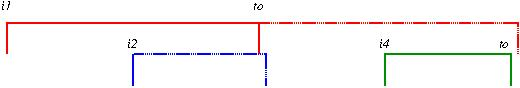
\includegraphics[width=.8\textwidth]{wiggling.jpg}
\end{center}

We partition all events in \red{blocks}\  that contains an input and all timeouts that it triggers.
A \red{race}\ occurs when right before an event some timer is $0$ and this event is not a timeout of that timer.

\vspace{1 em}
\red{Lemma}\ If there are no races we can wiggle any block.

\red{Lemma}\ Each race is won by one block. 

\red{Lemma}\ A block can lose only once.

\red{Lemma}\ Blocks are partially ordered by winning relation.

\red{Lemma}\ A block that doesn't win any race can be wiggled forward.


}

\frame{
\frametitle{Myhill-Nerode (1)}
Let $S$ be a set of feasible untimed behaviors. Then $S$ is
\begin{itemize}
\item
\red{prefix closed}: $\beta \beta' \in S \Longrightarrow \beta \in S$,
\item
\red{behavior deterministic}:
$\beta \xrightarrow{i/o_1, \rho_1} X_1 \in S \wedge \beta \xrightarrow{i/o_2, \rho_2} X_2 \in S \Longrightarrow o_1 = o_2 \wedge \rho_1 = \rho_2 \wedge X_1 = X_2$,
\item
\red{input complete}:
$\beta \in S \wedge i \in I \Longrightarrow \exists o, \rho, Y : \beta \xrightarrow{i/o, \rho} Y \in S$,
\item
\red{timeout complete}:
$\beta \in S \wedge x \mbox{ expirable after } \beta \Longrightarrow
\exists o, \rho, Y: \beta \xrightarrow{\toevent{x}/o, \rho} Y \in S$.
\end{itemize}
Behaviors $\beta, \beta' \in S$ are \red{equivalent}, notation $\beta \equiv_S \beta'$, iff 
for any untimed behavior
$\gamma$, $\beta \cdot \gamma \in S \Leftrightarrow \beta' \cdot \gamma \in S$.
}


\frame{
\frametitle{Myhill-Nerode (2)}

\red{Theorem}\\
Let $S$ be a set of feasible untimed behaviors over finite sets of inputs $I$, outputs $O$, and timers $Y$.
Then $S$ is the set of feasible untimed behaviors of an MMT $\M$ iff $S$ is nonempty, all untimed behaviors in $S$
start with the empty set of timers, $S$ is prefix closed, behavior deterministic, input complete, timeout complete,
and $\equiv_S$ has only finitely many equivalence classes (finite index).
}

\frame{
\frametitle{Learning Algorithm}

Based on Myhill-Nerode result we define an Angluin style learning algorithm for MMTs. Key idea: introduce membership queries for untimed behaviors and implement these via membership queries for timed words.

\vspace{1em}
\red{Challenge 1.}\  How to observe causality in timed word in practice? Different fractional parts for different inputs?  Wiggling?!

\vspace{1em}
\red{Challenge 2.}\  Figure out which timers are active in a state. May be resolved using \red{lookahead oracle}, as in the  Tomte tool. 

\vspace{1em}
Assuming a lookahead oracle and a teacher that answers equivalence queries, and considering the number of clocks as constant,
the number of queries is polynomial in size MMT.
}

\frame{
\frametitle{Conclusions and Future Work}

\begin{itemize}
\item
Everybody is using timed automata in which clocks run forward. It feels like driving on the wrong side of the road to study MMTs. But it is fun!
\item
MMTs constitute interesting modelling framework for which tractable learning algorithm exists.
\item
Future work: study various forms of timing uncertainty.
\item
Get rid of timer liveness assumption.
\item
Implement and apply to practical case studies.
\end{itemize}

}





\end{document}
